% ----------------------------------------------------
% Literature Review
% ----------------------------------------------------
\documentclass[class=report,11pt,crop=false]{standalone}
\input{../Style/ChapterStyle.tex}
\makenoidxglossaries

\newacronym{fm}{FM}{frequency modulation}
\newacronym{lora}{LoRa}{Long Range}
\newacronym{iot}{IOT}{Internet of Things}
\newacronym{fsk}{FSK}{Frequency Shift Keying}
\newacronym{chirp}{CHIRP}{Compressed High Intensity Radar Pulse}
\newacronym{atps}{ATPs}{Acceptance Test Protocols}
\newacronym{hal}{HAL}{Hardware Abstraction Layer}
\newacronym{oled}{OLED}{Organic Light Emitting Diode}
\newacronym{rssi}{RSSI}{Received Signal Strength Index}
\newacronym{uart}{UART}{Universal Asynchronous Receive and Transmit}
\newacronym{usb}{USB}{Universal Serial Bus}
\newacronym{css}{CSS}{Chirp Spread Spectrum}
\newacronym{i2c}{I2C}{Inter-Integrated Circuit}
\newacronym{spi}{SPI}{Serial Peripheral Interface}
\newacronym{gps}{GPS}{Global Positioning System}
\newacronym{nmea}{NMEA}{National Marine Electronics Association}
\newacronym{mac}{MAC}{Media Access Control}
\newacronym{sf}{SF}{Spreading Factor}
\newacronym{arr}{ARR}{Auto Reload Register}
\newacronym{sdr}{SDR}{Software Defined Radio}
\newacronym{pcb}{PCB}{Printed Circuit Board}
\newacronym{fdm}{FDM}{Frequency Division Multiplexing}


\newacronym{radar}{RADAR}{Radio Detection and Ranging}
\newacronym{ofdm}{OFDM}{Orthogonal Frequency Division Multiplexing}
\newacronym{tdm}{TDM}{Time Division Multiplexing}
\newacronym{tdma}{TDMA}{Time Division Multiple Access}
\newacronym{att}{AT\&T}{American Telephone and Telegraph Company}
\newacronym{usrp}{USRP}{Universal Software Radio Peripheral}
\newacronym{uct}{UCT}{University of Cape Town}


\begin{document}

\definecolor{colour8}{HTML}{ffd700}
\definecolor{colour7}{HTML}{ffb14e}
\definecolor{colour6}{HTML}{fa8775}
\definecolor{colour5}{HTML}{ea5f94}
\definecolor{colour4}{HTML}{cd34b5}
\definecolor{colour3}{HTML}{9d02d7}
\definecolor{colour1}{HTML}{0000ff}
\definecolor{colour2}{HTML}{1197ff}

% ----------------------------------------------------
\chapter{Literatures Review}\label{ch:Literature}
\section{Background}
As mentioned in chapter \ref{ch:Introduction}, thousands of weather balloons are launched every day to help meteorologists predict and research weather. The majority of these weather balloons operate around the 400 MHz frequency band \cite{ITURec}. These weather balloons have a small device called a radiosonde that hangs below the balloon itself and contains meteorological measurement devices \cite{noaa_radiosondes}. Most of these radiosonde devices record information about the temperature, pressure, relative humidity, and the position of the module itself using the \gls{gps} \cite{noaa_radiosondes}.


\section{LoRa Communication Standard}
LoRa is a fairly new communication standard that has become very popular over the last few years due to its ability to provide a platform for low data rate, wide-area transmissions. This has been particularly useful within the IOT world, due to many IOT systems requiring their transmissions of data to be low power and small in data packet size. The LoRa modulation scheme is also particularly cheap and easy to implement when compared to other communication protocols, which are not so well developed and maintained. This coupled with the ability of LoRa to transmit small amounts of data at low power, is why the LoRa protocol is being investigated for use in radiosondes. Before I can go any further, however, I need to make a distinction between LoRa and LoRaWAN. The barebones LoRa that is mostly discussed in this report, is only a physical layer method of wireless transport \cite{froehlich_what_2020}. This means that whenever LoRa is mentioned, most of the time what is being talked about is the physical transmission protocol that takes place in a point-to-point LoRa network. LoRaWAN on the other hand is an open, cloud-based protocol, designed and maintained by the LoRa Alliance, that enables devices to communicate wirelessly with LoRa \cite{froehlich_what_2020}. LoRaWAN is a \gls{mac} layer protocol built on top of LoRa modulation meaning that it is a software layer which defines how devices use the LoRa hardware, for example when they transmit, and the format of messages \cite{things_network_what_nodate}. For this report, whenever LoRa is mentioned, it refers to the physical layer of the LoRa protocol and not the MAC layer which is governed by LoRaWAN. 

\section{LoRa History}
The origins of LoRa begin in 2009, when two friends by the names of Nicolas Sornin and Olivier Seller, decided to explore the idea of encoding data using the \gls{css} technique as a base signal \cite{slats_brief_2020}. After some initial development on the idea, and after meeting their third business partner, François Sforza, the three of them decided to start a company called Cycleo, which was eventually acquired by Semtech only two years later in 2012, after Semtech were convinced by the viability of the technology \cite{slats_brief_2020}. With the help of Semtech, the three members of the original team developed the LoRa protocol into what it is known today. Today, Semtech hold all the major patents and other legal documents which gives them the right to design and produce products using the LoRa modulation technique.

\section{LoRa for Weather Balloons}
There is a handful of literature surrounding the use of the LoRa protocol for weather balloon applications. Two papers stick out above the rest, the papers are "LoRa Transmission System for Weather Balloons" by May Anne Valencia, Febus Reidj Cruz, and Raymart Balakit, from Mapua University, Manila, Philippines; and "A Custom Radiosonde Design for Environmental Measurements Over Maritime Areas" by Antonio Turi, Matteo Gemignani, and Salvo Marcuccio, from the University of Pisa, Pisa, Italy.

May Anne Valencia, Febus Reidj Cruz, and Raymart Balakit talk about how the cost of radiosonde modules is a prohibiting factor in how many atmospheric observations can be made by countries. They mention how in the Philippines, radiosonde modules are launched from seven sites around the country, twice per day. Each radiosonde costs approximately \$200.00, which as of the end of October 2023, is roughly R3780.00 \cite{lora_transmission_system_for_weather_balloons}. The low-altitude radiosonde modules cost approximately \$155, which as of the end of October 2023, is roughly R2930.00 \cite{lora_transmission_system_for_weather_balloons}. They go on to successfully design and implement a LoRa-based radiosonde system, with successful transmissions from the module up to an altitude of roughly 10km \cite{lora_transmission_system_for_weather_balloons}.

Antonio Turi, Matteo Gemignani, and Salvo Marcuccio discuss their attempt at using the LoRa protocol to design a weather balloon module over maritime areas. They discuss the process of designing a complete measurement system that includes a time stamp, latitude, longitude, GNSS altitude, horizontal speed, number of GNSS satellites in view, air temperature, air pressure, relative humidity, and barometric altitude \cite{a_custom_radiosonde_design_for_environmental_measurements_over_maritime_areas}. This is more in line with the sort of data collection that this report outlines. They were able to successfully complete a test over a distance of 43km, using an omnidirectional antenna on the transmit side, and a directional yagi antenna on the receiver side \cite{a_custom_radiosonde_design_for_environmental_measurements_over_maritime_areas}. They also noted the positive effects that came from transmitting without any objects within the fresnel zonse of the link between the transmitter and the receiver.

\section{Fresnel Zones}
When dealing with line-of-sight communication links, it is important to keep any obstacles out of an elliptical region between the two links, which is called the fresnel zone \cite{editorial_team_everything_rf_what_2018}. Figure \ref{fig:fresnelzones} below gives a visual understanding of what fresnel zones look like. 

\begin{figure}[H]
    \centering
    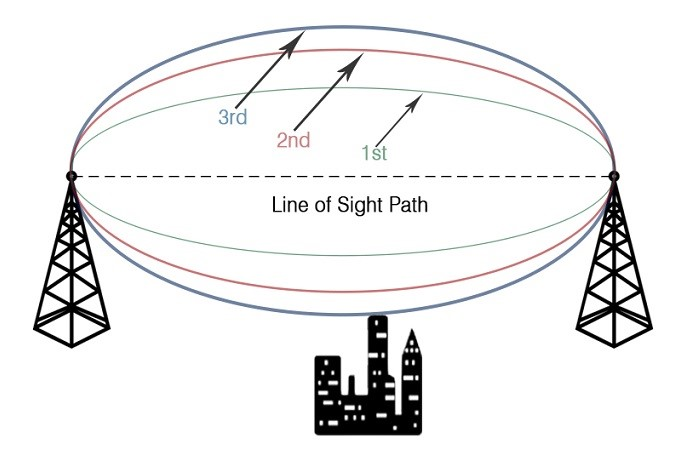
\includegraphics[width=0.5\linewidth]{../Images/fresnelZones.jpeg}
    \caption{Diagram of fresnel zones \cite{editorial_team_everything_rf_what_2018}}
    \label{fig:fresnelzones}
\end{figure}

Fresnel zones are generally broken up into multiple ellipses that correspond to a specific fresnel zone. For example, zone 1 in the above image is denoted by the label "1st", zone 2 by "2nd" and so on. Obstacles in the 1st Fresnel Zone will create signals that will be 0 to 90 degrees out of phase, 90 to 270 degrees out of phase in the 2nd zone, 270 to 450 degrees out of phase in the 3rd zone and so on \cite{4gon_solutions_4gon_nodate}.

Equation \ref{eq:fresnelzoneradius} below shows the calculation required to determine the radius of the fresnel zone for communication links.

\begin{equation}
    r=\sqrt{\frac{nd_{1}d_{2}\lambda}{d_{1}+d_{2}}} \label{eq:fresnelzoneradius}
\end{equation}

In this equation $n$ is the fresnel zone number, $d_{1}$ is the distance from antenna 1 to point P along the direct pathway between the two antennas, $d_{2}$ is the distance from point P to antenna 2, along the same direct pathway from antenna 1 to antenna 2, $\lambda$ is the frequency at which the link is operating, and $r$ is the fresnel zone radius at point P.

\section{LoRa Theory of Operation}
To understand the theory of how LoRa works, the first step is to understand \gls{fsk} at a broad level. This modulation scheme is outlined in the following section.
\subsection{Frequency Shift Keying}
FSK is a form of frequency modulation that involves encoding a symbol into a specific frequency \cite{How_LoRa_Modulation_really_works_long_range_communication_using_chirps_2021}. The most simple form of a system like this would be a binary transmission system. A system like this would have a designated frequency for a 1, and a designated frequency for a 0. For example, if $f_{0}$ corresponded to a higher relative frequency than $f_{1}$, and in this scheme, $f_{0}$ was encoded as a "1", and $f_{1}$ was encoded as a "0", then the time domain signal for the four symbols, "1010", would be as shown in figure \ref{fig:FSK1} below. This is assuming that the transmission and receiving modules are synchronised and both have a measurement period of T.

\begin{figure}[H]
\centering
\begin{tikzpicture}
  \begin{axis}[
    xlabel={Time},
    ylabel={Amplitude},
    axis lines=middle,
    xmin=0, xmax=4, ymin=-1.5, ymax=1.5,
    xtick={0,1,2,3,4},
    ytick={-1,0,1},
    xticklabels={0,$1T$,$2T$,$3T$,$4T$},
    yticklabels={-1,0,1},
    grid=both,
    major grid style={dashed, gray!50},
    width=12cm, height=6cm,
    y axis line style={<->}, % Adds arrows at both ends
  ]
  
  % Higher and lower frequency graphs
  \addplot[colour1, domain=0:1, samples=100, thick] {sin(500*pi*x)};
  \addplot[colour3, domain=1:2, samples=100, thick] {sin(225*pi*x)};
  \addplot[colour1, domain=2:3, samples=100, thick] {sin(500*pi*x)};
  \addplot[colour3, domain=3:4, samples=100, thick] {sin(225*pi*x)};

  % Labels
  \node[black, anchor=west] at (0.4, -1.3) {$f_{0}$};
  \node[black, anchor=west] at (1.4, -1.3) {$f_{1}$};
  \node[black, anchor=west] at (2.4, -1.3) {$f_{0}$};
  \node[black, anchor=west] at (3.4, -1.3) {$f_{1}$};

  \end{axis}
\end{tikzpicture}
\caption{1 Bit/Symbol Frequency Shift Keying}
\label{fig:FSK1}
\end{figure}

This is a very good base system, however, only being able to send one bit at a time is not very useful for most purposes. This idea can be expanded to incorporate more symbols. The above example in figure \ref{fig:FSK1} only has two symbols encoded into frequencies $f_{0}$ and $f_{1}$. The number of symbols encoded can be increased by declaring more frequencies as specific symbols. For example, with eight unique signals, you can encode 3 bits per symbol. This means that one can encode the numbers 0-7. In figure \ref{fig:FSK2} below, I have defined eight different frequencies, ranging from $f_{0}$ to $f_{7}$ to represent numbers 0-7.

\begin{figure}[H]
\centering
\begin{tikzpicture}
  \begin{axis}[
    xlabel={},
    ylabel={},
    axis lines=middle,
    xmin=0, xmax=8, ymin=-1.5, ymax=1.5,
    xtick={0,1,2,3,4,5,6,7,8},
    ytick={-1,0,1},
    xticklabels={,,,,,,,,},
    yticklabels={-1,0,1},
    grid=both,
    major grid style={dashed, gray!50},
    width=16cm, height=6cm,
    y axis line style={<->}, % Adds arrows at both ends
  ]
  
  % Higher and lower frequency graphs
  \addplot[colour1, domain=0:1, samples=100, thick] {sin(100*pi*x)};
  \addplot[colour2, domain=1:2, samples=100, thick] {sin(200*pi*x)};
  \addplot[colour3, domain=2:3, samples=100, thick] {sin(300*pi*x)};
  \addplot[colour4, domain=3:4, samples=100, thick] {sin(400*pi*x)};
  \addplot[colour5, domain=4:5, samples=100, thick] {sin(500*pi*x)};
  \addplot[colour6, domain=5:6, samples=100, thick] {sin(600*pi*x)};
  \addplot[colour7, domain=6:7, samples=100, thick] {sin(700*pi*x)};
  \addplot[colour8, domain=7:8, samples=100, thick] {sin(800*pi*x)};

  % Labels
  \node[black, anchor=west] at (0.4, -1.3) {$f_{0}$};
  \node[black, anchor=west] at (1.4, -1.3) {$f_{1}$};
  \node[black, anchor=west] at (2.4, -1.3) {$f_{2}$};
  \node[black, anchor=west] at (3.4, -1.3) {$f_{3}$};
  \node[black, anchor=west] at (4.4, -1.3) {$f_{4}$};
  \node[black, anchor=west] at (5.4, -1.3) {$f_{5}$};
  \node[black, anchor=west] at (6.4, -1.3) {$f_{6}$};
  \node[black, anchor=west] at (7.4, -1.3) {$f_{7}$};

  \node[black, anchor=west] at (0.3, 1.3) {000};
  \node[black, anchor=west] at (1.3, 1.3) {001};
  \node[black, anchor=west] at (2.3, 1.3) {010};
  \node[black, anchor=west] at (3.3, 1.3) {011};
  \node[black, anchor=west] at (4.3, 1.3) {100};
  \node[black, anchor=west] at (5.3, 1.3) {101};
  \node[black, anchor=west] at (6.3, 1.3) {110};
  \node[black, anchor=west] at (7.3, 1.3) {111};

  \end{axis}
\end{tikzpicture}
\caption{8 Bit/Symbol Frequency Definitions}
\label{fig:FSK2}
\end{figure}

Using this method, we could transmit the following four numbers, or symbols, "4", "7", "2", and "3". This transmission is shown in figure \ref{fig:FSK3} below.

\begin{figure}[H]
\centering
\begin{tikzpicture}
  \begin{axis}[
    xlabel={},
    ylabel={},
    axis lines=middle,
    xmin=0, xmax=4, ymin=-1.5, ymax=1.5,
    xtick={0,1,2,3,4},
    ytick={-1,0,1},
    xticklabels={0,$1T$,$2T$,$3T$,$4T$},
    yticklabels={-1,0,1},
    grid=both,
    major grid style={dashed, gray!50},
    width=16cm, height=6cm,
    y axis line style={<->}, % Adds arrows at both ends
  ]
  
  % Higher and lower frequency graphs
  \addplot[colour1, domain=0:1, samples=100, thick] {sin(500*pi*x)};
  \addplot[colour2, domain=1:2, samples=100, thick] {sin(800*pi*x)};
  \addplot[colour3, domain=2:3, samples=100, thick] {sin(300*pi*x)};
  \addplot[colour4, domain=3:4, samples=100, thick] {sin(400*pi*x)};

  % Labels
  \node[black, anchor=west] at (0.4, -1.3) {$f_{4}$};
  \node[black, anchor=west] at (1.4, -1.3) {$f_{7}$};
  \node[black, anchor=west] at (2.4, -1.3) {$f_{2}$};
  \node[black, anchor=west] at (3.4, -1.3) {$f_{3}$};


  \node[black, anchor=west] at (0.3, 1.3) {100};
  \node[black, anchor=west] at (1.3, 1.3) {111};
  \node[black, anchor=west] at (2.3, 1.3) {010};
  \node[black, anchor=west] at (3.3, 1.3) {011};

  \end{axis}
\end{tikzpicture}
\caption{8 Bit/Symbol Frequency Shift Keying}
\label{fig:FSK3}
\end{figure}

Assuming that the transmission and receiver side of the system are set up correctly and synchronised, then as you can see, each symbol is transmitted for a specific period. Since both systems are synchronised, the receiving side can determine which frequency is being sent and what symbol is being sent via correlation which determines exactly what frequency is being received \cite{How_LoRa_Modulation_really_works_long_range_communication_using_chirps_2021}. Another way to visualise this signal transmission is with a waterfall plot. A waterfall plot shows the frequency domain and time domain in a single diagram, allowing the user to see what frequencies are being sent on the frequency spectrum over time. For the transmission of the symbols "4", "7", "2", and "3", the waterfall plot will look as shown in figure \ref{fig:FSK4} below.


\begin{figure}[H]
\centering
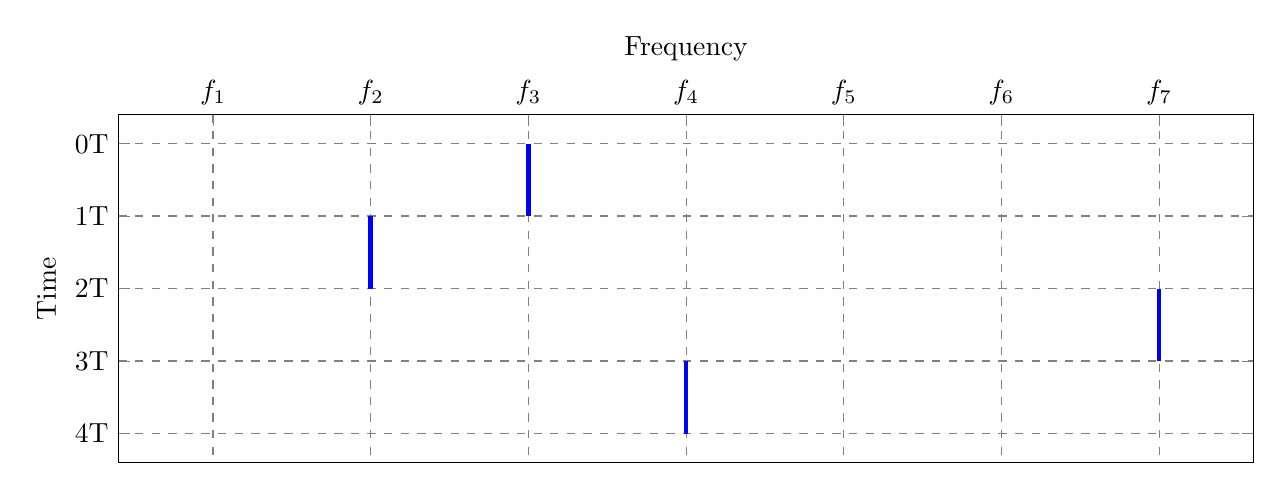
\begin{tikzpicture}
  \begin{axis}[
    xlabel={Frequency},
    ylabel={Time},
    xtick={0,1,2,3,4,5,6,7}, % Adjust xticks according to your data
    xticklabels={$f_{0}$,$f_{1}$,$f_{2}$,$f_{3}$,$f_{4}$,$f_{5}$,$f_{6}$,$f_{7}$},
    ytick={0,0.1,0.2,0.3,0.4,0.5}, % Adjust xticks according to your data
    yticklabels={0T,1T,2T,3T,4T,5T},
    grid=both,
    major grid style={dashed, black!50}, % Customize major gridlines here
    minor grid style={dotted, black!20}, % Customize minor gridlines here
    width=16cm,
    height=6cm,
    xtick pos=top,
    y dir=reverse,
  ]
  \addplot[blue, ultra thick, smooth] coordinates {(1,0.0) (1,0.0)};
  \addplot[blue, ultra thick, smooth] coordinates {(2,0.1) (2,0.2)};
  \addplot[blue, ultra thick, smooth] coordinates {(3,0.0) (3,0.1)};
  \addplot[blue, ultra thick, smooth] coordinates {(4,0.3) (4,0.4)};
  %\addplot[blue, ultra thick, smooth] coordinates {(5,0.3) (5,0.5)};
  %\addplot[blue, ultra thick, smooth] coordinates {(6,0.3) (6,0.5)};
  \addplot[blue, ultra thick, smooth] coordinates {(7,0.2) (7,0.3)};
  \end{axis}
\end{tikzpicture}
\caption{Waterfall plot of a transmission of the "4723" symbols}
\label{fig:FSK4}
\end{figure}

As you can see, the various frequencies that correspond to the different symbols are shown at the different time periods in which they occur on the transmission side, with the first symbols to be received being shown at the bottom of the waterfall plot. 

One of the issues with a system like this is that as you increase the size of the symbols that you are transmitting, the more frequencies you need to encode the data. As the number of frequencies increases, it becomes harder for the receiving side to decode the data \cite{How_LoRa_Modulation_really_works_long_range_communication_using_chirps_2021}. For example, if you wanted to transmit 8 bit symbols, which would be a common need for many projects, then the system would require 256 distinct frequencies. Given the same bandwidth for transmission, one can see how having more frequencies to assign will decrease the amount of bandwidth between each frequency band, therefore making the decoding of the sent signal harder, because it will become more difficult to determine the difference between the various signals. A way to get around this problem is to use the full bandwidth available for each symbol that you want to transmit, and this is where the chirp comes in.

\subsection{The Chirp}\label{sec:chirps}
A \gls{chirp} is simply a sinusoidal wave that experiences a frequency change with time \cite{lora_symbol_generation_2023}. A chirp wave has a constant amplitude in the time domain, with a varying frequency over time. There are two main types of simple chirp, the up-chirp and the down-chirp. An up-chirp increases in frequency over time, and a down-chirp decreases with frequency over time. An example of both can be seen in figure \ref{fig:CHIRP3} below.


\begin{figure}[H]
\centering
\begin{subfigure}{.5\textwidth}
    \centering
\begin{tikzpicture}
  \begin{axis}[
    xlabel={Time},
    ylabel={Amplitude},
    axis lines=middle,
    xmin=0, xmax=1, ymin=-1.5, ymax=1.5,
    xtick={0,1},
    ytick={-1,0,1},
    %xticklabels={0,$1T$},
    yticklabels={-1,0,1},
    grid=both,
    major grid style={dashed, gray!50},
    width=6cm, height=6cm,
    y axis line style={<->}, % Adds arrows at both ends
    xlabel style={at={(ticklabel cs:1.04)}, anchor=south west, yshift=17pt}, % Move entire x-axis label to the right
  ]
  
  % Higher and lower frequency graphs
  \addplot[colour1, domain=0:1, samples=1000, thick] {sin(2*pi*(500/2)*x^2)};


  \end{axis}
\end{tikzpicture}
\caption{Up-Chirp}
\label{fig:CHIRP1}
\end{subfigure}%
\begin{subfigure}{.5\textwidth}
    \centering
\begin{tikzpicture}
  \begin{axis}[
    xlabel={Time},
    ylabel={Amplitude},
    axis lines=middle,
    xmin=0, xmax=1, ymin=-1.5, ymax=1.5,
    xtick={0,1},
    ytick={-1,0,1},
    xticklabels={0,$1T$},
    yticklabels={-1,0,1},
    grid=both,
    major grid style={dashed, gray!50},
    width=6cm, height=6cm,
    y axis line style={<->}, % Adds arrows at both ends
    xlabel style={at={(ticklabel cs:1.04)}, anchor=south west, yshift=17pt}, % Move entire x-axis label to the right
  ]
  
  % Higher and lower frequency graphs
  \addplot[colour1, domain=0:1, samples=1000, thick] {sin(2*pi*(1000 - 499*x)*x)};


  \end{axis}
\end{tikzpicture}
\caption{Down-Chirp}
\label{fig:CHIRP2}
\end{subfigure}%
\caption{Up-Chirp and Down-Chirp}
\label{fig:CHIRP3}
\end{figure}

These chirps form the basis for the way in which the LoRa system encodes data for transmission. An example of these chirps on a waterfall plot can be seen in figure \ref{fig:CHIRP4} below. This figure shows an up-chirp between times 2T and 3T, and a down-chirp between times 0T and 1T, which span a bandwidth B, centred on frequency $f_{0}$. Each chirp in the figure had a period of 1T and in between each chirp transmission, a 1T period elapsed without any transmission happening at all.


\begin{figure}[H]
\centering
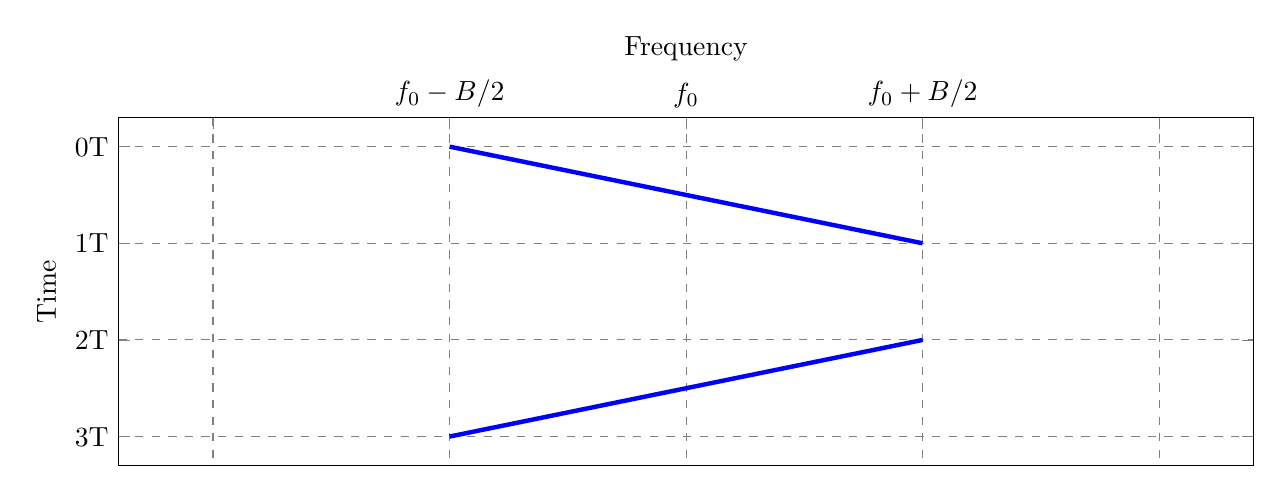
\begin{tikzpicture}
  \begin{axis}[
    xlabel={Frequency},
    ylabel={Time},
    xtick={0,1,2,3,4,5,6,7}, % Adjust xticks according to your data
    xticklabels={ , , ,$f_{0}-B/2$,$f_{0}$,$f_{0}+B/2$, , },
    ytick={0,0.1,0.2,0.3,0.4,0.5}, % Adjust xticks according to your data
    yticklabels={0T,1T,2T,3T,4T,5T},
    grid=both,
    major grid style={dashed, black!50}, % Customize major gridlines here
    minor grid style={dotted, black!20}, % Customize minor gridlines here
    width=16cm,
    height=6cm,
    xtick pos=top,
    y dir=reverse,
  ]
  %\addplot[blue, ultra thick, smooth] coordinates {(1,0.0) (1,0.0)};
  \addplot[blue, ultra thick, smooth] coordinates {(2,0.0) (2,0.0)};
  \addplot[blue, ultra thick, smooth] coordinates {(3,0.3) (5,0.2)};
  \addplot[blue, ultra thick, smooth] coordinates {(5,0.1) (3,0.0)};
  %\addplot[blue, ultra thick, smooth] coordinates {(5,0.3) (5,0.5)};
  \addplot[blue, ultra thick, smooth] coordinates {(6,0.0) (6,0.0)};
  %\addplot[blue, ultra thick, smooth] coordinates {(7,0.0) (7,0.0)};
  \end{axis}
\end{tikzpicture}
\caption{Waterfall plot of a transmission of an up-chirp and a down-chirp}
\label{fig:CHIRP4}
\end{figure}

As can be seen in the figure above, the chirp signal either starts at a lower frequency and increases in frequency with time or starts at a higher frequency and decreases in frequency with time. Whether or not a chirp increases or decreases in frequency with time depends on whether it is an up or down chirp. The difference between the starting frequency and the ending frequency is called the bandwidth. This CHIRP forms the basis for LoRa transmissions. The idea of a LoRa transmission is that the actual data packet is encoded in up-chirps that are transmitted. Apart from other information that is sent with each transmission, which is discussed in section \ref{sec:loradatapackets}, a rough idea of what a LoRa transmission looks like can be seen in figure \ref{fig:loratransmissionwithdiscontinuities} below. As can be seen in this figure, there exist discontinuities as time moves forward. These discontinuities are where the data in a LoRa transmission is encoded. For instance, a discontinuity at the position as shown between time periods 3T and 2T could be assigned a symbol value of 0, a discontinuity at the position as shown between time periods 2T and 1T could be assigned a symbol value of 1, and a discontinuity at the position as shown between time periods 1T and 0T could be assigned a symbol value of 2. Therefore, the transmission in the below figure, would be the transmission of the symbols "0", "1", and "2", in that order.

\begin{figure}[H]
\centering
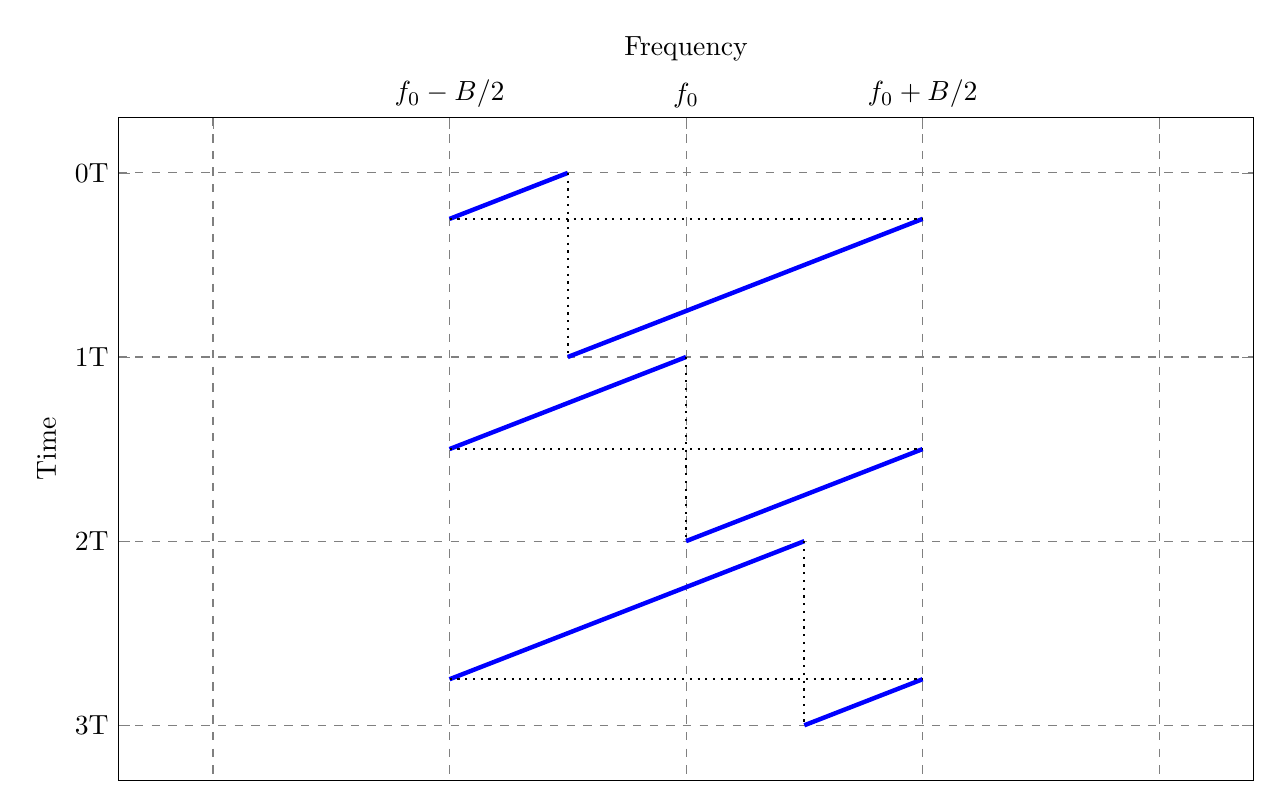
\begin{tikzpicture}
  \begin{axis}[
    xlabel={Frequency},
    ylabel={Time},
    xtick={0,1,2,3,4,5,6,7}, % Adjust xticks according to your data
    xticklabels={ , , ,$f_{0}-B/2$,$f_{0}$,$f_{0}+B/2$, , },
    ytick={0,1,2,3,4,5}, % Adjust xticks according to your data
    yticklabels={0T,1T,2T,3T,4T,5T},
    grid=both,
    major grid style={dashed, black!50}, % Customize major gridlines here
    minor grid style={dotted, black!20}, % Customize minor gridlines here
    width=16cm,
    height=10cm,
    xtick pos=top,
    y dir=reverse,
  ]
  \addplot[blue, ultra thick, smooth] coordinates {(2,0) (2,0)};

    % Last LoRa transmission
  \addplot[blue, ultra thick, smooth] coordinates {(3,0.25) (3.5,0)};
  \addplot[blue, ultra thick, smooth] coordinates {(3.5,1) (5,0.25)};
  \addplot[black, thick, dotted] coordinates {(3.5,0) (3.5,1)};
  \addplot[black, thick, dotted] coordinates {(3,0.25) (5,0.25)};

  % Middle LoRa transmission
  \addplot[blue, ultra thick, smooth] coordinates {(3,1.5) (4,1)};
  \addplot[blue, ultra thick, smooth] coordinates {(4,2) (5,1.5)};
  \addplot[black, thick, dotted] coordinates {(4,1) (4,2)};
  \addplot[black, thick, dotted] coordinates {(3,1.5) (5,1.5)};

    %First LoRa Transmission
  \addplot[blue, ultra thick, smooth] coordinates {(3,2.75) (4.5,2)};
  \addplot[blue, ultra thick, smooth] coordinates {(4.5,3) (5,2.75)};
  \addplot[black, thick, dotted] coordinates {(4.5,2) (4.5,3)};
  \addplot[black, thick, dotted] coordinates {(3,2.75) (5,2.75)};
  
  \addplot[blue, ultra thick, smooth] coordinates {(6,0) (6,0)};
  
  \end{axis}
\end{tikzpicture}
\caption{Waterfall plot of a transmission of an up-chirp and a down-chirp with discontinuities}
\label{fig:loratransmissionwithdiscontinuities}
\end{figure}

It must be noted that a LoRa transmission has many more features than the example in the above figure, however, this understanding of how the LoRa protocol encodes symbols in the discontinuities of frequency up-chirps is a very good base level of knowledge to understand the workings of the LoRa transmission protocol. 

\subsection{Bandwidth}
The bandwidth for a LoRa transmission is simply the difference between the minimum frequency and the maximum frequency in a transmission. For example, in figure \ref{fig:loratransmissionwithdiscontinuities} above, the bandwidth is $(f_{0}+B/2) - (f_{0}-B/2)$. For many LoRa transmission modules, the most common bandwidth values are 7.8 kHz, 10.4 kHz, 15.6 kHz, 20.8 kHz, 31.25 kHz, 41.7 kHz, 62.5 kHz, 125 kHz, 250 kHz, or 500 kHz. 

\subsection{Spreading Factor}
Now that the simple chirp signal has been explained, the next idea that must be explored is the \gls{sf} of a LoRa transmission. The spreading factor is the number that denotes the speed at which the up or down chirps travel across the available bandwidth \cite{lora_spreading_factor_explained_2022}. Since the data in a LoRa transmission is encoded into these chirps, there is a direct relationship between the spreading factor and the data rate achievable of a LoRa transmission. The available spreading factors for the popular SX1278 LoRa module are 7, 8, 9, 10, 11, and 12. With each increase in the spreading factor, the time it takes for a chirp to propagate the entirety of the available bandwidth increases by a factor of two. This effect is illustrated in figure \ref{fig:CHIRP5} below. In this figure, the bandwidth, B, of the LoRa transmission is set to a known value, and the transmission occurs on a centre frequency of $f_{0}$. The only parameter that is being changed is the spreading factor. In the case of the below figure, the first transmission that occurs is equivalent to the highest spreading factor transmission, and the most recent transmission that occurs is equivalent to the lowest spreading factor transmission. The most recent transmission, that being the lowest spreading factor transmission, has a period of 1T, and the last transmission received, that being the highest spreading factor transmission, has a period of 32T.


\begin{figure}[H]
\centering
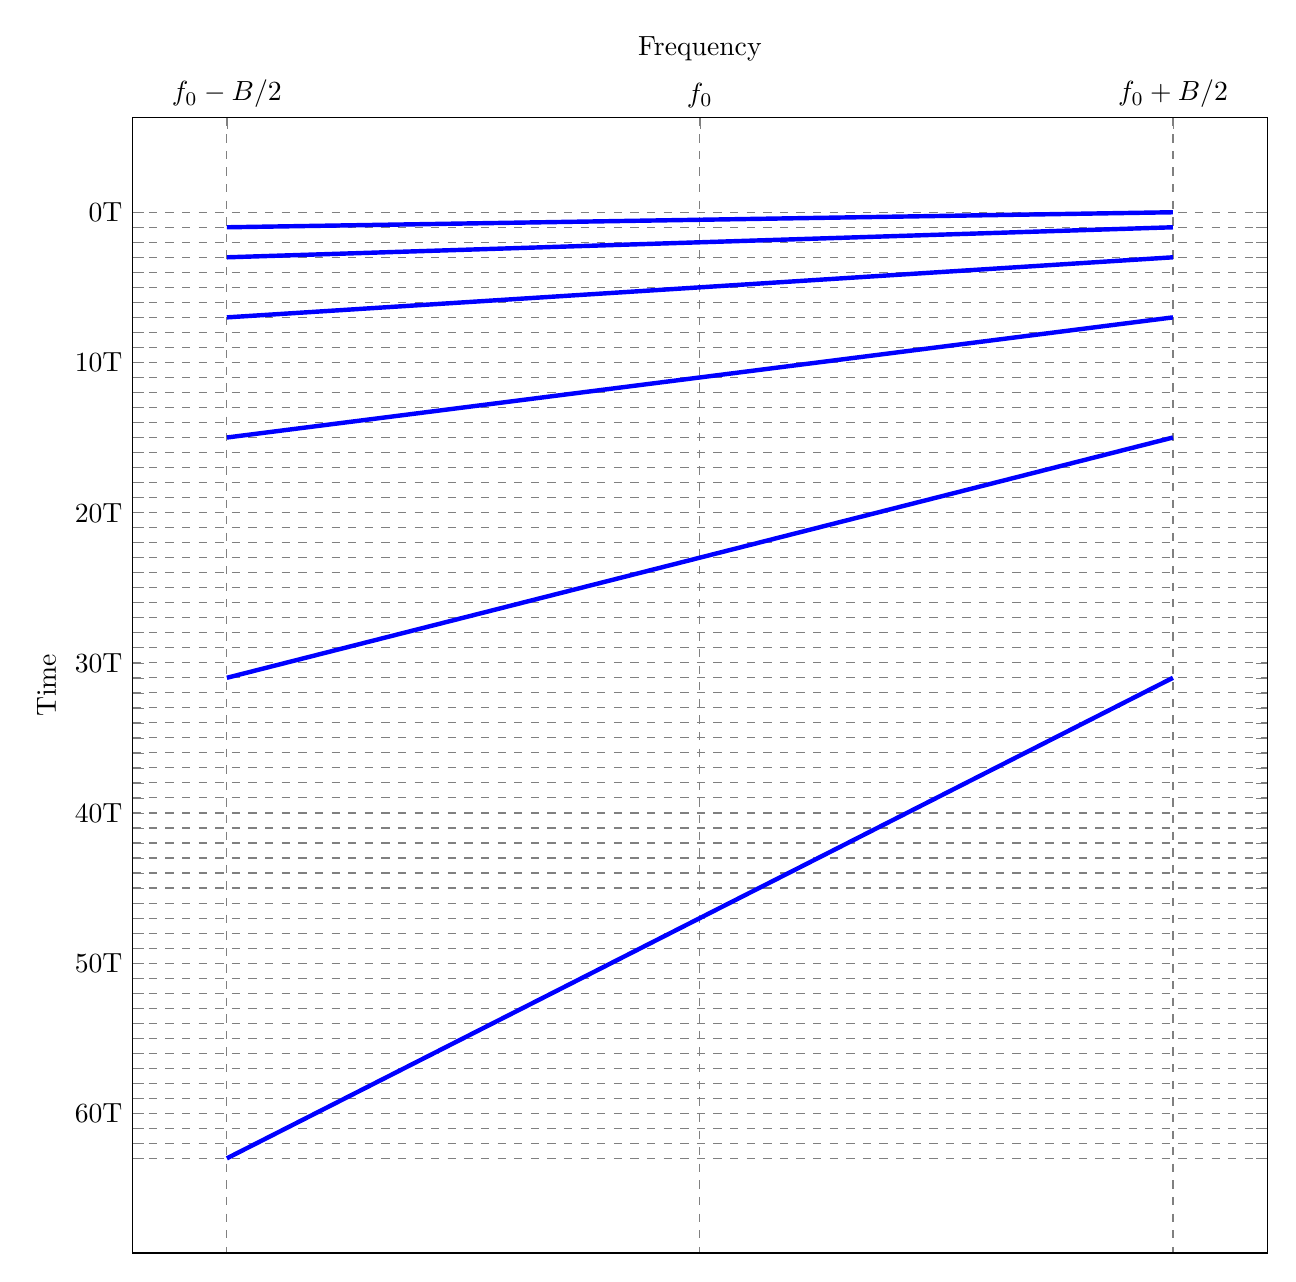
\begin{tikzpicture}
  \begin{axis}[
    xlabel={Frequency},
    ylabel={Time},
    xtick={1,2,3}, % Adjust xticks according to your data
    xticklabels={$f_{0}-B/2$,$f_{0}$,$f_{0}+B/2$},
    ytick={0,1,2,3,4,5,6,7,8,9,10,11,12,13,14,15,16,17,18,19,20,21,22,23,24,25,26,27,28,29,30,31,32,33,34,35,36,37,38,39,40,41,42,43,44,45,46,47,48,49,50,51,52,53,54,55,56,57,58,59,60,61,62,63}, % Adjust xticks according to your data
    yticklabels={0T,,,,,,,,,,10T,,,,,,,,,,20T,,,,,,,,,,30T,,,,,,,,,,40T,,,,,,,,,,50T,,,,,,,,,,60T},
    grid=both,
    major grid style={dashed, black!50}, % Customize major gridlines here
    minor grid style={dotted, black!20}, % Customize minor gridlines here
    width=16cm,
    height=16cm,
    xtick pos=top,
    y dir=reverse,
  ]

  \addplot[blue, ultra thick, smooth] coordinates {(1,1) (3,0)};%1
  \addplot[blue, ultra thick, smooth] coordinates {(1,3) (3,1)};%2
  \addplot[blue, ultra thick, smooth] coordinates {(1,7) (3,3)};%4
  \addplot[blue, ultra thick, smooth] coordinates {(1,15) (3,7)};%8
  \addplot[blue, ultra thick, smooth] coordinates {(1,31) (3,15)};%16
  \addplot[blue, ultra thick, smooth] coordinates {(1,63) (3,31)};%32

  \end{axis}
\end{tikzpicture}
\caption{Various spreading factors for an up-chirp}
\label{fig:CHIRP5}
\end{figure}


As can be seen in the above figure, as the spreading factor increases, the time that it takes to send one chirp increases. Therefore, it now becomes clear why the spreading factor has an influence on the data rate achievable in a LoRa transmission because it actually changes the rate at which the modulated chirps occur. In the above figure, I have made the smallest spreading factor correspond to a period of 1T, however, in reality, each symbol has a length in time of $\frac{2^{SF}}{BW}$ \cite{decodinglora_2020}.

\subsection{LoRa Data Packets}\label{sec:loradatapackets}
Now that the basic LoRa transmission parameters have been explained, the LoRa packet structure can be examined. All of the following packet contents are encoded in the up-chirps and down-chirps discussed previously in section \ref{sec:chirps}. Overall, LoRa packets have two different modes, those two modes are explicit and implicit header mode. Explicit header mode is usually the default mode used by LoRa transmitters, such as the SX1278. Explicit header mode allows for variable-length packets to be sent because information about the packet length is contained within the header that is sent, whereas implicit header mode only allows for specific lengths of packets that have been predefined to be sent. An example of a LoRa packet that utilises the explicit header mode can be seen below in figure \ref{fig:loraexplicitpacket}. 

\begin{figure}[H]
    \centering
    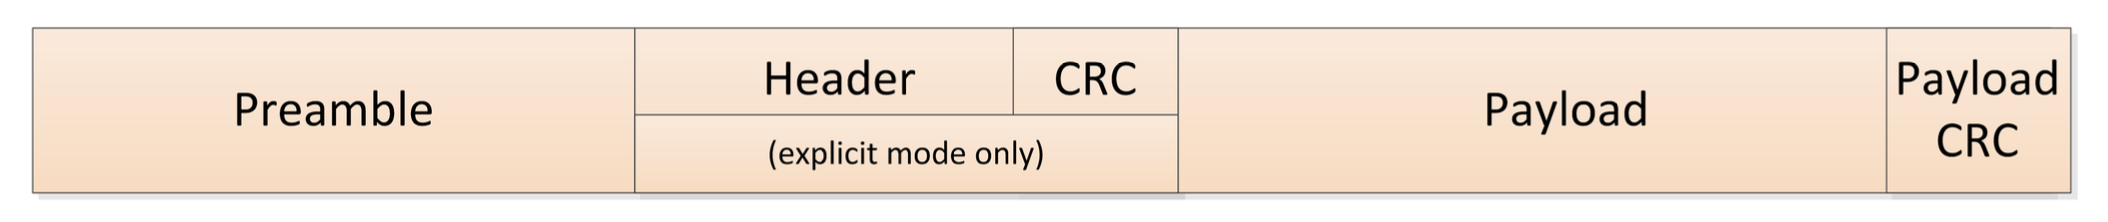
\includegraphics[width=0.8\linewidth]{../Images/explicitPacket.png}
    \caption{LoRa Explicit Packet \cite{SX1278}}
    \label{fig:loraexplicitpacket}
\end{figure}

As can be seen, the LoRa packet consists of a preamble first. The preamble is used to synchronize the receiver with the transmitter. The radio transmitter will add another 4.25 symbols resulting in a final preamble length of 8 + 4.25 = 12.25 symbols \cite{thingsnetwork_lora}. Next, the header is transmitted which contains information about the packet of data itself and information about the cyclic redundancy check that the LoRa system utilises. After this, the actual packet of data is sent. Lastly, some more cyclic redundancy data is sent that contains an error-detecting code for correcting errors in the payload messages \cite{thingsnetwork_lora}.

\subsection{LoRa Transmission Parameters}\label{sec:loratransmissionparameters}
Any transmission that abides by the LoRa protocol is governed by certain parameters. These parameters are examined for the common SX1278 LoRa transmitter in this section. 

\subsubsection{Symbol Rate and Symbol Time}
One of the first parameters to understand is the symbol rate $R_{S}$. $R_{S}$ is defined by equation \ref{eq:symbolrate} below \cite{SX1278}.

\begin{equation}
    R_{S}=\frac{BW}{2^{SF}} \label{eq:symbolrate}
\end{equation}

The symbol rate is the amount of symbols that can be transmitted per second. Essentially, it denotes how many symbols, which are the up-chirps with modulated discontinuities as seen in figure \ref{fig:loratransmissionwithdiscontinuities}, can be sent per second. From equation \ref{eq:symbolrate} above, we can deduce that if the spreading factor stays constant, then an increasing bandwidth will increase the symbol rate. We can also see that if bandwidth is constant, then an increasing spreading factor decreases the symbol rate.

The converse of the symbol rate is the symbol time. This is defined as follows in equation \ref{eq:symboltime} \cite{SX1278}.
\begin{equation}
T_{S}=\frac{1}{R_{S}} \nonumber
\end{equation}
\begin{equation}
\therefore T_{S}=\frac{1}{(\frac{BW}{2^{SF}})} \nonumber
\end{equation}
\begin{equation}
\therefore T_{S}=\frac{2^{SF}}{BW} \label{eq:symboltime}
\end{equation}

\subsubsection{Preamble Time}
The time that a Lora transmission spends on the preamble part of the transmission is defined in equation \ref{eq:preambletime} below \cite{SX1278}:

\begin{equation}
    T_{preamble}=(n_{preamble}+4.25)\times T_{S} \label{eq:preambletime}
\end{equation}

where $n_{preamble}$ is the number of preamble symbols, which is a parameter that most LoRa transmitters have as customizable. For most transmitters, the standard number of preamble symbols is 8.

\subsubsection{Payload Time}
The payload time is the time it takes to transmit the actual payload of the LoRa transmission. The payload time is defined in equation \ref{eq:payloadtime} below  \cite{SX1278}:

\begin{equation}
    T_{payload}=n_{payload}\times T_{S} \label{eq:payloadtime}
\end{equation}

where $n_{payload}$ is equivalent to the following  \cite{SX1278}:

\begin{equation}
    n_{payload}=8+max\left(ceil\left(\frac{(8PL-4SF+28+16CRC-20IH)}{4(SF-2DE)}\right)(CR+4),0\right) \label{eq:npayload}
\end{equation}
where 
\begin{itemize}
    \item PL is the payload size in bytes (between 1 and 255 bytes)
    \item SF is the spreading factor
    \item CRC is whether or not the cyclic redundancy check is on. (1 for yes and 0 for no)
    \item IH is whether or not a header is present (0 for yes and 1 for no)
    \item DE indicates whether or not the low data rate optimization mode is enabled (1 for yes and 0 for no)
    \item CR is the coding rate. 1 indicates a coding rate of 4/5, 2 indicates a coding rate of 4/6 and so on
\end{itemize}
Therefore, the full equation for the payload time is the combination of equation \ref{eq:payloadtime} and equation \ref{eq:npayload}. This combination can be seen in equation \ref{eq:payloadtimefinal} below.

\begin{equation}
    T_{payload}=\left(8+max\left(ceil\left(\frac{(8PL-4SF+28+16CRC-20IH)}{4(SF-2DE)}\right)(CR+4),0\right)\right)\times T_{S} \label{eq:payloadtimefinal}
\end{equation}

\subsubsection{Packet Time}
The entire time that one packet takes to transmit can therefore be defined by equation \ref{eq:packettime} below.
\begin{equation}
    T_{packet}=T_{preamble}+T_{payload} \label{eq:packettime}
\end{equation}

Substituting equation \ref{eq:preambletime} and equation \ref{eq:payloadtimefinal} into the above equation gives the overall packet time equation. This can be seen below.

\begin{equation}
    T_{packet}=T_{S}\left([n_{preamble}+4.25]+\left[8+max\left(ceil\left(\frac{(8PL-4SF+28+16CRC-20IH)}{4(SF-2DE)}\right)(CR+4),0\right)\right]\right)
\end{equation}

\section{Critique of Literature}
There seems to be ample literature that goes into detail about the usage of the LoRa protocol, especially from the hobbyist maker community. However, something that was noted, was the lack of in-depth detail about the signal processing and inner workings of the LoRa modulation scheme. This is primarily due to the fact that the LoRa protocol is a patented technology with a lot of the literature surrounding the exact inner workings of the system not available to the general public. There is however enough information out there to build a broad understanding of the operation of the system to a level that is necessary to perform the desired experiments outlined in this report.

The literature surrounding the usage of the LoRa protocol for weather balloons is somewhat well documented, however, none of the previous examples of this explicit use case included testing into what the optimal LoRa parameters would be for the transmission of the data from the weather balloon to the base station.




% ----------------------------------------------------
\ifstandalone
\bibliography{../Bibliography/References}
\printnoidxglossary[type=\acronymtype,nonumberlist]
\fi
\end{document}
% ----------------------------------------------------